\documentclass[12pt,a4paper,draft]{report}
\usepackage[utf8]{inputenc}
\usepackage[french]{babel}
\usepackage[T1]{fontenc}
\usepackage{amsmath}
\usepackage{amsfonts}
\usepackage{amssymb}
\usepackage{graphicx}
\usepackage{pdfpages}
\usepackage[nottoc,section]{tocbibind}

\renewcommand{\thesection}{\arabic{section}}

\graphicspath{{pictures/}}

\begin{document}

\begin{titlepage}
\author{Alexandre \textsc{Marin}\\ Master Mathématiques et applications Sorbonne Université\\ Parcours Ingénierie Mathématique\\ Majeure Ingénierie Mathématique Pour l'Entreprise}
\date{24/06 -- 30/10/2020\\ Institut Fran\c{c}ais du P\'etrole \'Energies Nouvelles\\ Site de Rueil-Malmaison}
\title{Développement d’une bibliothèque de structures et algorithmes pour un mailleur polyédrique}
\maketitle
\end{titlepage}

\begin{titlepage}
\section*{Remerciements}
\end{titlepage}

\begin{titlepage}
\tableofcontents
\end{titlepage}


\section{Introduction}
%1 page
%ouverture
%annonce du plan
%position du stagiaire dans l'entreprise
Ce document est le rapport de mon stage qui a eu lieu à l'Institut Français du Pétrole \'Energies Nouvelles (IFPEN), et clôture donc ma seconde année de master à Sorbonne Université.

Ma position de stagiaire a été la suivante~: j'ai été intégré dans la direction scientifique \emph{Sciences et Technologies du Numérique}, et plus précisément dans le département \emph{Informatique Scientifique} du site de Rueil-Malmaison de IFPEN.

Ce rapport présente d'abord succinctement le déroulement du stage, expose ensuite le contexte du stage en présentant l'entreprise, puis la mission du stage est détaillée et une quatrième partie apporte la conclusion.

\section{Déroulement du stage}
%un paragraphe par mois
%une ou deux pages
Le premier mois du stage a été consacré à la découverte des locaux, à certaines formations obligatoires pour les nouveaux salariés (comme la formation sécurité) et à l'installation de logiciels nécessaires pour le stage. \`A la fin du mois de juillet, j'avais pris en main l'environnement de développement intégré QtCreator, une structure de données en demi-arêtes pour des maillages bidimensionnels était programmée en C++ et des maillages de Delaunay pouvaient être générés.

Pendant le deuxième mois, le code C++ a ensuite été réorganisé dans le but d'ajouter plus facilement d'autres fonctionnalités comme le calcul de triangulations de Delaunay contraintes. De nombreux tests ont aussi été effectués pour vérifier la stabilité des programmes ainsi que la qualité des résultats.

\section{Contexte et données générales}
%2-3 pages
L'Institut Français du Pétrole -- \'Energies Nouvelles (IFPEN) est une entreprise du groupe du même nom : il s'agit d'un établissement public de recherche et de formation dans les domaines de l'énergie, du transport et de l'environnement, placé sous la tutelle du ministre chargé de l'énergie. IFPEN est financé environ à moitié par l'\'Etat et crée lui-même plus de 50\% de son budget, notamment en valorisant le travail issu de la recherche. L'entreprise est présente sur deux sites : l'un à Rueil-Malmaison en \^Ile-de-France et l'autre à Solaize en Auvergne-Rhône-Alpes.

En 2019, IFPEN comptait $1\ 633$ salariés à temps plein, dont $1\ 136$ ingénieurs et techniciens R\&I (Recherche et Innovation), ainsi que près de $200$ allocataires de recherche, postdoctorants et stagiaires. Son budget atteignait $283,3$\textrm{M}\texteuro. IFPEN déposait aussi $185$ brevets et est à l'origine de plus de $600$ publications scientifiques et communications à congrès.

IFPEN conçoit et développe des procédés, des équipements et des logiciels qui concernent quatre domaines : la mobilité durable, les énergies renouvelables, les hydrocarbures responsables, et le climat/l'environnement. Dans le domaine climat et environnement, l'une des problématiques est par exemple le captage, le stockage et l'utilisation du CO$_2$. Il s'agit de proposer aux industries lourdes (sidérurgie, cimenterie, raffinage, chimie, pétrochimie) des technologies pour réduire massivement leurs émissions de CO$_2$.

IFPEN collabore avec d'autres instituts de recherche et industries dans le cadre de partenariats qui sont de différents types. IFPEN est ses partenaires financent conjointement un projet de recherche et définissent les règles de propriétés des résultats grâce aux contrats de recherches bilatéraux, aux consortiums dont certains sont des Joint Industry Project (JIP) : IFPEN y opère le programme R\&I et conserve la propriété industrielle. IFPEN participe aussi à des projets de recherche collaborative qui bénéficient de soutiens publics

La plupart des entités de IFPEN, que l'on peut voir sur la figure \ref{ifpen_org}, se répartissent dans deux ensembles : les directions de recherche, qui rassemblent les compétences scientifiques, et les directions fonctionnelles, comme les ressources humaines, les finances ou le juridique.

Les programmes de recherche sont menés à travers des projets pouvant faire intervenir plusieurs directions de recherche et fonctionnelles. Ces mêmes projets sont pilotés par l'un des cinq centres de résultats qui s'occupent également de leur valorisation industrielle.

On trouve aussi dans l'entreprise une école d'ingénieurs, IFP School, ainsi que la direction générale. Il y a enfin un conseil d'administration, composé de seize membres dont quatre sont des représentants de l'\'Etat venant des ministères de l'énergie, de l'industrie, du budget et de la recherche.

\section{Mission du stage}
%objectifs
%travail fait
%résultats
%problèmes

\section{Conclusion}

\section{Annexes}

\begin{center}
\begin{figure}[htbp]
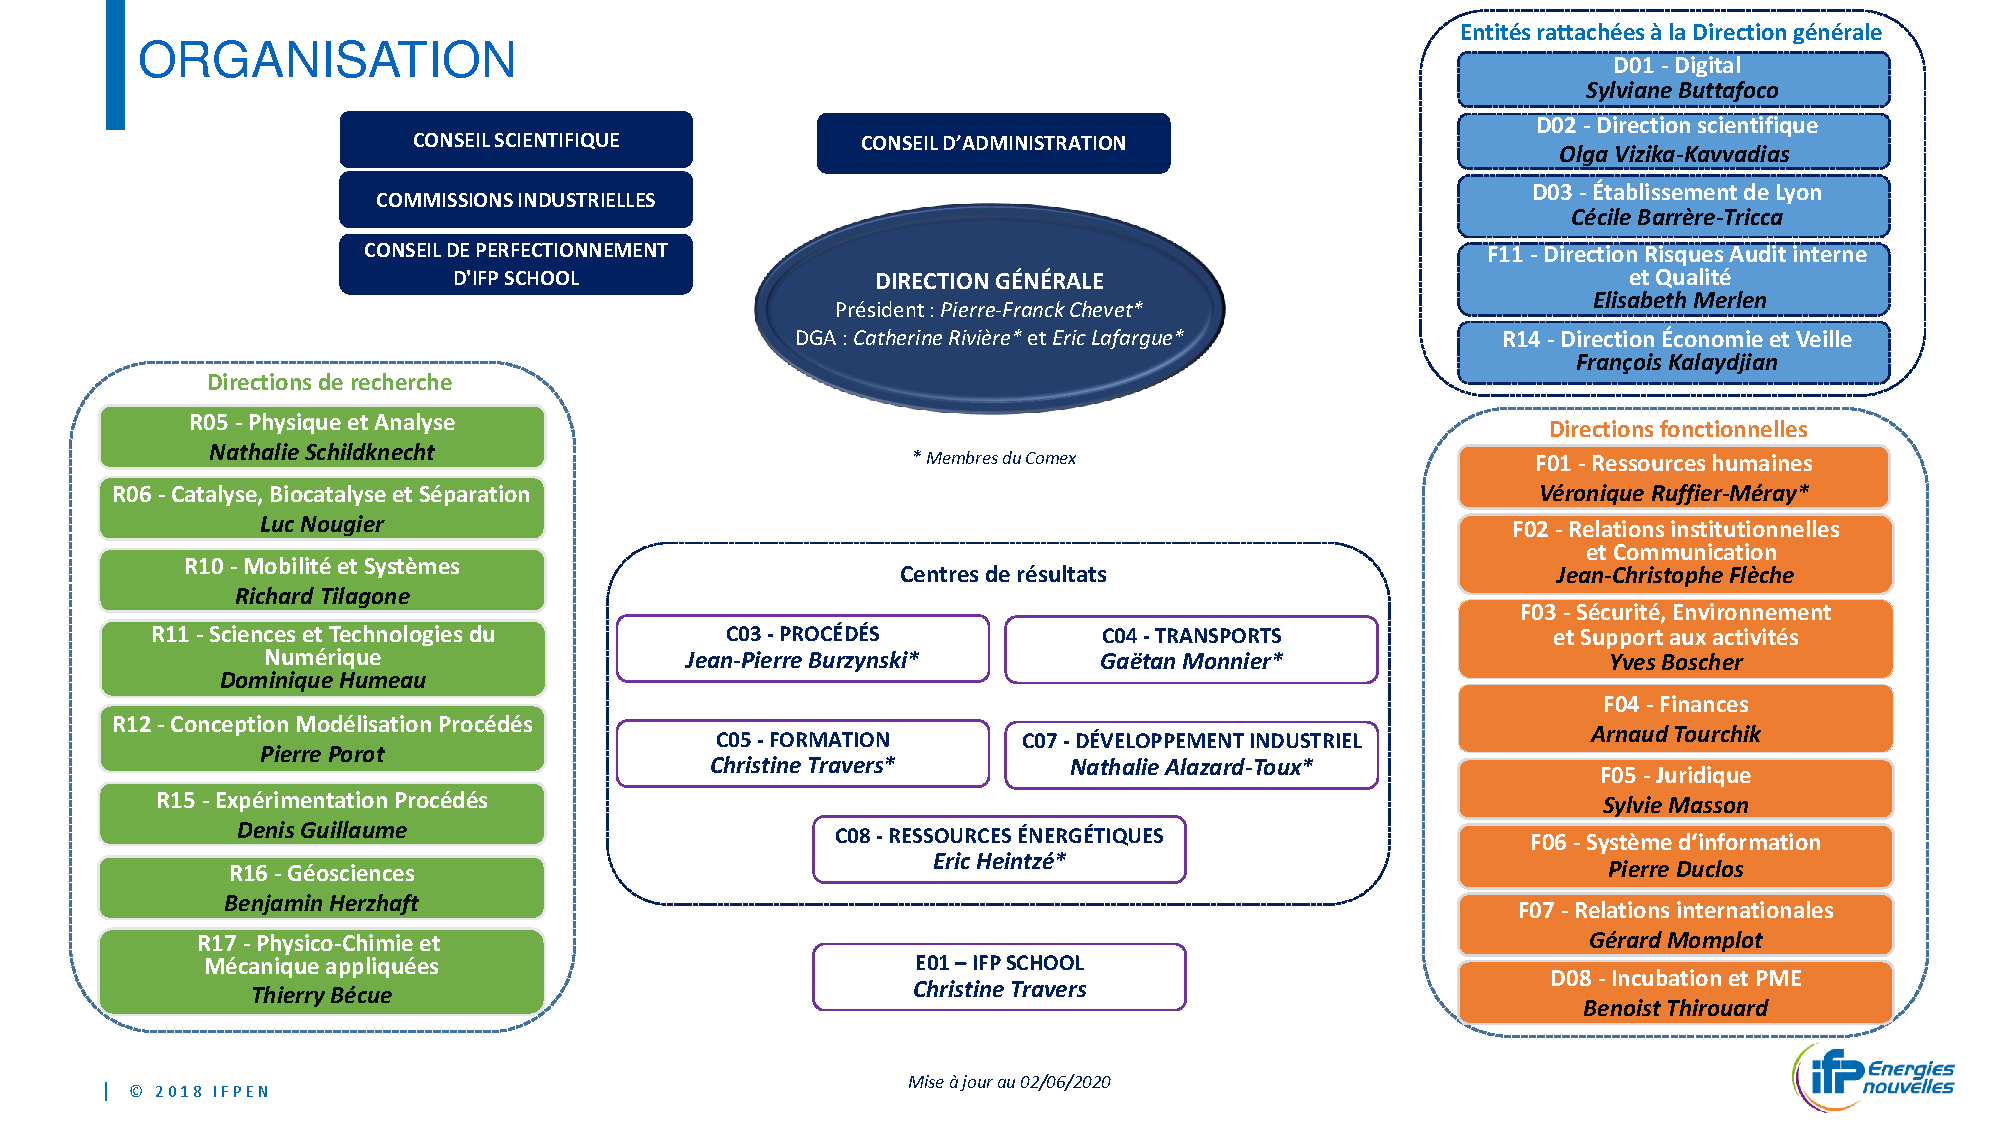
\includegraphics[scale=0.6, angle=90]{vf-schema-organisation-ifpen-marguerite.pdf}
\caption{Schéma de l'organisation de l'IFPEN (source : intranet de l'IFPEN)}
\label{ifpen_org}
\end{figure}
\end{center}
\clearpage

\nocite{*}
%bibliography
\bibliographystyle{plain}
\bibliography{doc}

\end{document}